\subsection{Fantasia3D}\label{fantasia3D}

The model proposed by \citeauthor{chen2023fantasia3d} takes a different approach to generating 3D models from text input, in particular by disentangling geometry and appearance in the generated 3D models.
This method offers a more detailed rendering quality compared to conventional Neural Radiance Fields (NeRFs), which use volume rendering to combine the learning of surface geometry with pixel colors. This conventional approach limits effective surface recovery, lacking the capability to track the surface of an object and tune detailed material and texture. In contrast, Fantasia3D achieves more realistic outputs with its hybrid scene representation of DMTet, ``which maintains a deformable tetrahedral grid and a differentiable mesh extraction layer; deformation can thus be learned through the layer to explicitly control the shape generation'' \citep{chen2023fantasia3d}

In the geometry stage, Fantasia3D relies on a Deformable Mesh Tetrahedralization (DMTet), which parametrizes the 3D geometry as a Multi-Layer Perceptron (MLP) \(\Psi\). Initially, Fantasia3D renders and encodes surface normals and object masks extracted from DMTet. However, in later stages, the model refines its approach by using only the rendered normal map for shape encoding \citep{chen2023fantasia3d}. The default initialization of DMTet is an ellipsoid, but the model also accepts custom inputs.

\begin{figure}[ht]
  \centering
    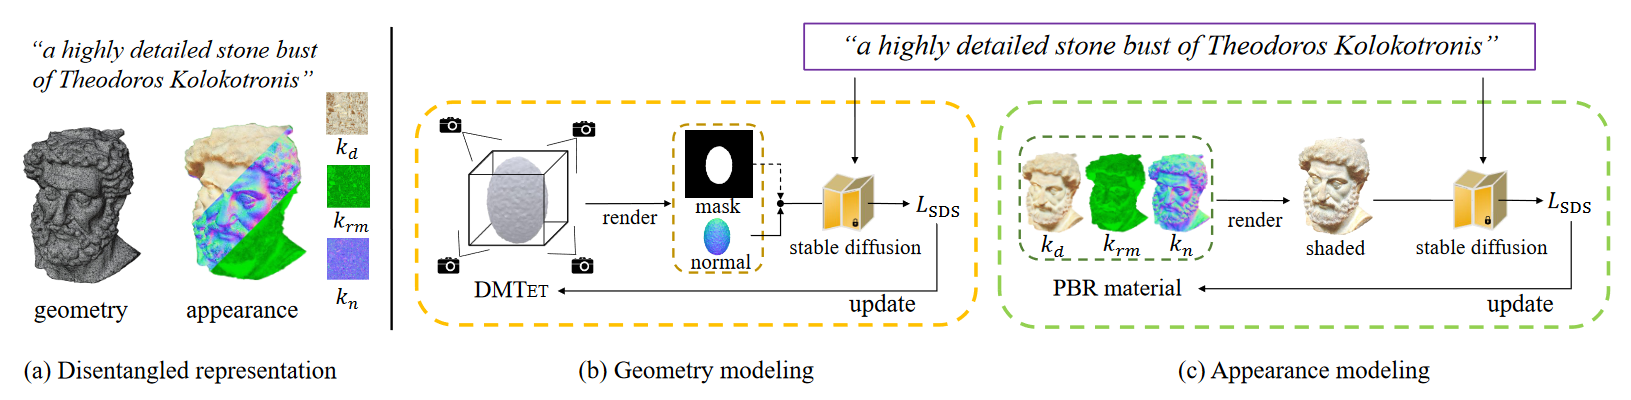
\includegraphics[width=1\columnwidth]{figures/Fantasia3D.png}
    \caption{Overview of Fantasia3D's workflow as given in \citep{chen2023fantasia3d}, disentangling geometry from appearance modeling and iteratively enhancing the quality using a refinement process.}\label{fig:figureFantasia}
\end{figure}

In the Appearance stage of Fantasia3D, the aim is to achieve photorealism in surface rendering using the DMTet from the geometry stage, by integrating the Physically-Based Rendering (PBR) material model \citep{mcauley2012practical}. This model includes the diffuse term \( k_d \), the combined roughness and metallic term \( k_{rm} \), and the normal variation \( k_n \) \citep{chen2023fantasia3d}. To predict these material parameters, a Multilayer Perceptron (MLP) denoted as \( \Gamma \) is used. The process involves the application of the formula \((k_d, k_{rm}, k_n) = \Gamma(\beta(p); \gamma)\) by \citeauthor{chen2023fantasia3d}, where \( \beta(p) \) represents the surface properties at a specific point \( p \) and \( \gamma \) indicates the network parameters. The rendering of each pixel's color within this framework involves the integration of incident light and the Bidirectional Reflectance Distribution Function (BRDF) \citep{chen2023fantasia3d}. The BRDF plays a crucial role in accurately depicting how light reflects off different surfaces, with its parameters directly influenced by the material properties \( (k_d, k_{rm}, k_n) \). Additionally, the appearance generated in this stage is converted into 2D texture maps. These maps are aligned with the UV maps produced, ensuring a seamless and realistic texturing of the 3D model surfaces.

Both MLPs (\(\Gamma\) for appearance and \(\Psi\) for geometry) undergo a refinement process, using a pre-trained Stable Diffusion model \citep{rombachStableDiffusion}. This model improves the capabilities of \(\Gamma\) and \(\Psi\), ensuring that they accurately interpret and render 3D shapes and textures. A key aspect of this refinement is the use of Score Distillation Sampling (SDS) loss \citep{mildenhallNERF} for optimization. This step allows the model to evaluate and adjust its rendering based on how accurately it replicates the true image of Stable Diffusion. By iterating this process for multiple viewpoints, the model continually improves its accuracy in rendering photorealistic images, ensuring that the final output is as close to the actual image as possible.

Fantasia3D offers a high degree of user interactivity, permitting the incorporation of both custom and predefined generic 3D shapes, thus greatly enhancing the versatility and user engagement in the content creation process. The separation of geometry and appearance generation also ensures compatibility with widely-used graphics engines \citep{chen2023fantasia3d}. Despite its capabilities in creating high-quality 3D models from textual descriptions, Fantasia3D encounters specific challenges. One notable limitation is its struggle with accurately generating complex geometries like hair, fur, and grass \citep{chen2023fantasia3d}. Furthermore, the model is currently not able to generate complete scenes as focus is currently lying on individual object generation \citep{chen2023fantasia3d}.